\documentclass{tufte-handout}

\title{3.2 Polynomials and their graphs}

\author[AW]{Ammon Washburn}

\usepackage{graphicx} % allow embedded images
  \setkeys{Gin}{width=\linewidth,totalheight=\textheight,keepaspectratio}
  \graphicspath{{graphics/}} % set of paths to search for images
\usepackage{amsmath}  % extended mathematics
\usepackage{booktabs} % book-quality tables
\usepackage{units}    % non-stacked fractions and better unit spacing
\usepackage{multicol} % multiple column layout facilities
\usepackage{lipsum}   % filler text
\usepackage[inline]{enumitem}
\usepackage{wrapfig}
\usepackage{fancyvrb} % extended verbatim environments
  \fvset{fontsize=\normalsize}% default font size for fancy-verbatim environments
  \usepackage{tikz}

% Standardize command font styles and environments
\newcommand{\doccmd}[1]{\texttt{\textbackslash#1}}% command name -- adds backslash automatically
\newcommand{\docopt}[1]{\ensuremath{\langle}\textrm{\textit{#1}}\ensuremath{\rangle}}% optional command argument
\newcommand{\docarg}[1]{\textrm{\textit{#1}}}% (required) command argument
\newcommand{\docenv}[1]{\textsf{#1}}% environment name
\newcommand{\docpkg}[1]{\texttt{#1}}% package name
\newcommand{\doccls}[1]{\texttt{#1}}% document class name
\newcommand{\docclsopt}[1]{\texttt{#1}}% document class option name
\newenvironment{docspec}{\begin{quote}\noindent}{\end{quote}}% command specification environment

\newtheorem{mydef}{Definition}
\providecommand{\floor}[1]{\left \lfloor #1 \right \rfloor }

\begin{document}
\maketitle

\begin{abstract}
Be familiar with polynomials of any degree and know what their graph looks like from just knowing the equation
\end{abstract}

\section{Polynomials}
Same definition as before
\begin{mydef}
A polynomial is an equation of the form $p(x) = a_n x^n + a_{n-1} x^{n-1} + \cdots + a_1 x + a_0$ where $a_n \neq 0$.
\end{mydef}

Again $n$ should be an integer.  All the $a_i$s are called the coefficients of the polynomial.  $a_0$ is the constant coefficient or many times the constant term (Since $x^0 = 1$). $a_n$ is called the leading coefficient while $a_n x^n$ is called the leading term.

\subsection{Graphing monomials}

\begin{marginfigure}
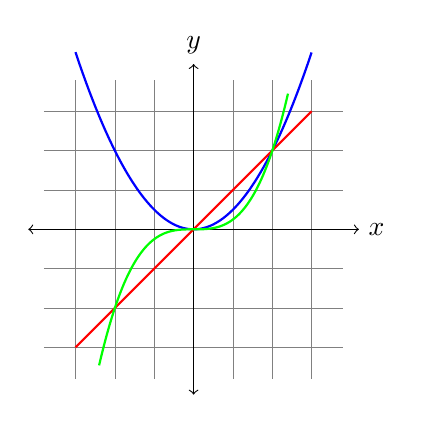
\begin{tikzpicture}
	\draw[very thin,color=gray,step=0.5] (-1.9,-1.9) grid (1.9,1.9);
	\draw[<->] (-2.1,0) -- (2.1,0) node[right] {$x$};
	\draw[<->] (0,-2.1) -- (0,2.1) node[above] {$y$};
	\draw[thick,smooth,samples=100,domain=-1.5:1.5,-,color=blue] plot (\x, {pow(\x,2)});
    \draw[thick,smooth,samples=100,domain=-1.5:1.5,-,color=red] plot (\x, {\x});
    \draw[thick,smooth,samples=100,domain=-1.2:1.2,-,color=green] plot (\x, {pow(\x,3)});
\end{tikzpicture}
\end{marginfigure}

Mononmials are functions that are like this $w(x) = x^n$.  For even $n$ then the graphs looks like a flatter quadratic (near the origin) and for odd $n$ it looks like a flatter cubic.  Be sure to know what their graphs and their transformations look like.

\subsection{End Behavior}
\begin{minipage}{.50\textwidth}
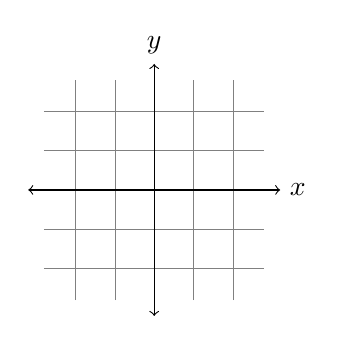
\begin{tikzpicture}
	\draw[very thin,color=gray,step=0.5] (-1.4,-1.4) grid (1.4,1.4);
	\draw[<->] (-1.6,0) -- (1.6,0) node[right] {$x$};
	\draw[<->] (0,-1.6) -- (0,1.6) node[above] {$y$};
\end{tikzpicture}
\end{minipage}
\begin{minipage}{.50\textwidth}
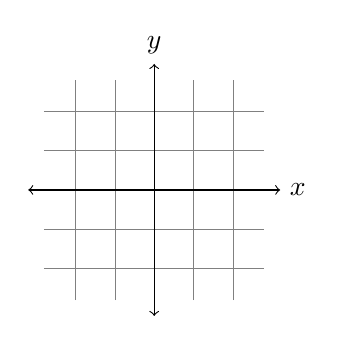
\begin{tikzpicture}
	\draw[very thin,color=gray,step=0.5] (-1.4,-1.4) grid (1.4,1.4);
	\draw[<->] (-1.6,0) -- (1.6,0) node[right] {$x$};
	\draw[<->] (0,-1.6) -- (0,1.6) node[above] {$y$};
\end{tikzpicture}
\end{minipage}
\begin{minipage}{.50\textwidth}
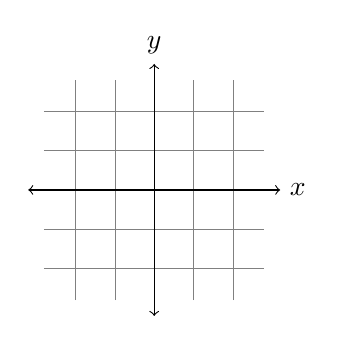
\begin{tikzpicture}
	\draw[very thin,color=gray,step=0.5] (-1.4,-1.4) grid (1.4,1.4);
	\draw[<->] (-1.6,0) -- (1.6,0) node[right] {$x$};
	\draw[<->] (0,-1.6) -- (0,1.6) node[above] {$y$};
\end{tikzpicture}
\end{minipage}
\begin{minipage}{.50\textwidth}
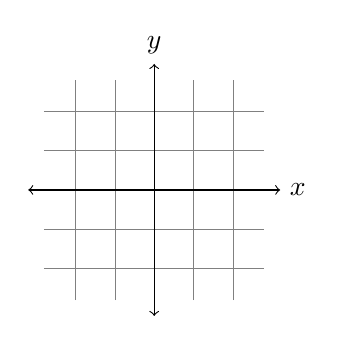
\begin{tikzpicture}
	\draw[very thin,color=gray,step=0.5] (-1.4,-1.4) grid (1.4,1.4);
	\draw[<->] (-1.6,0) -- (1.6,0) node[right] {$x$};
	\draw[<->] (0,-1.6) -- (0,1.6) node[above] {$y$};
\end{tikzpicture}
\end{minipage}

\subsection{Multiplicity of Zeros}
If you have your polynomial in root form it should look like this: $r(x) = (x-r_1)^{n_1}(x-r_2)^{n_2}\ldots(x-r_k)^{n_k}$ then $x=r_i$ is a root of multiplicity $n_i$.

\medskip

\begin{minipage}{.55\textwidth}
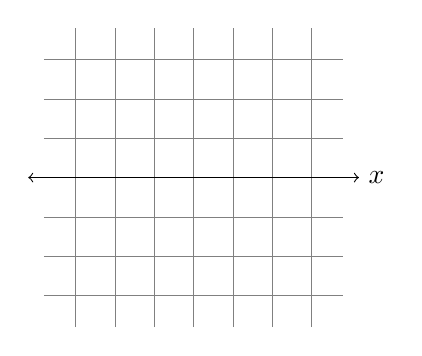
\begin{tikzpicture}
	\draw[very thin,color=gray,step=0.5] (-1.9,-1.9) grid (1.9,1.9);
	\draw[<->] (-2.1,0) -- (2.1,0) node[right] {$x$};
\end{tikzpicture}
\end{minipage}
\begin{minipage}{.55\textwidth}
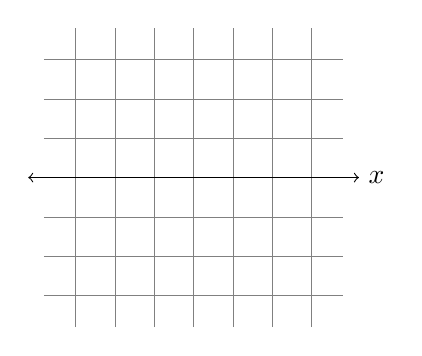
\begin{tikzpicture}
	\draw[very thin,color=gray,step=0.5] (-1.9,-1.9) grid (1.9,1.9);
	\draw[<->] (-2.1,0) -- (2.1,0) node[right] {$x$};
\end{tikzpicture}
\end{minipage}

\subsection{Graphing polynomials}

\begin{enumerate}
\item Find the zeros of the polynomial and their multiplicities
\item Find the end behavior and put them on the farthest zeros
\item Fill in the remaining spots using multiplicities
\end{enumerate}

Consider $u(x) = -x(x-2)^2(x+5)^3$. Zeros and their multiplicities: x= 0, 1; x=2,2; x=-5,3. End Behavior: Leading term is $-x^6$ so both point down.

\subsection{Examples}

\begin{align*}
f(x) &= (x-2)(x-4) & g(x) = (x-2)^2(x-4) \\ 
h(x) &= -(x-2)(x-4) & e(x) = -(x-2)(x-4)^2
\end{align*}

\subsection{Local Maximums and Minimums}

Linear functions have no local max or mins.  Quadratic functions have just one.  Cubics could have at most two.

A degree $n$ polynomial can have at most $n-1$ local maxs or mins.




\end{document}
